%
% Categorifying the zx-calculus
% Introduction
% qpl submission
%

\section{Introduction}
\label{sec:Introduction}

Compositionality is increasingly
becoming recognized as 
a viable point of view
from which to study 
complex systems such as 
those found in physics
	\cite{AbramCoecke_CatSemanticQuantum}, 
computer science 
	\cite{SassoneSobocinski_PetriNets}, 
and biology 
	\cite{BaezFongPollard_CompMarkovProcesses}.  
The focus is on 
connecting together smaller, 
simpler systems.  
The word `compositionality' suggests 
the relevancy of category theory.
This is indeed the case.
In fact, this paper
fits into a 
larger project of
establishing suitable categorical frameworks
in which to study composable systems
\cite{BaezCoyaFong_Props,
BaezFong_CompPassLinNets,
BaezFongPollard_CompMarkovProcesses,
BaezPollard_CompFrameRxNets,
Cicala_SpansCospans,
CicalaCourser_BicatSpansCospan,
Pollard_OpenMarkov}.
Open diagrams and diagrammatic languages
are typical players in compositional approaches. 
In our context, the adjective `open' is 
an established term
\cite{Dixon_OpenGraphs,
Merry_BangGraphs,
Pollard_OpenMarkov}
referring to a structure equipped with 
chosen inputs and outputs. 
The primary advantage of
open diagrams 
is the ability to work
within a more intuitive syntax.
Such diagrams are typically 
constructed with graph or 
topological string-like objects.  
Occasionally, additional data 
is attached to nodes, edges, or strings 
as needed. 
For example, open Markov chains
	\cite{Pollard_OpenMarkov}
use graphs whose nodes are 
labeled with a \emph{population} 
and edges with the rate at which 
the population of the source node 
shifts to the target node.  

Another common feature shared 
between diagrammatic languages is 
the notion of equality.  
Formal languages are often
equipped with a collection of rewrite rules.
For us, a rewrite rule is an equivalence relation
on diagrams stating when we can
replace a diagram $D$ with diagram $D'$.
This is our equality. 

Currently, syntax for diagrammatic calculi 
are usually captured with 1-categories
by encoding diagrams as morphisms
and diagram connection by composition. 
As mentioned above,
rewrite rules provide a notion of
equality between diagrams. 
However, 1-categorical frameworks squash 
the information contained in a rewrite rule.
That is, there is no way to reconstruct 
a rewrite rule from an equality. 
To more fully capture a system, 
rewrite rules ought to have better
representation in our syntax.
We accomplish this is by 
including them as 2-cells in a bicategory.  

What should such a bicategory look like? 
The 0-cells should 
communicate whether a pair of diagrams
can be connected.
Taking 0-cells to be sets, 
then a 1-cell $D \from x \to y$ is 
a diagram whose set of inputs is $x$ 
and set of outputs is $y$. 
Hence, we can connect to $D$ any
diagram whose inputs are $y$ or 
outputs are $x$.  
The 2-cells $D \Rightarrow D'$ are 
rules that rewrite $D$ into $D'$.  

To better envision such a bicategory, 
consider a hypothetical system
modeled by a directed graph $D$. 
Suppose that we would like $D$ 
to have inputs $I$ and outputs $O$, 
each subsets of the $D$-nodes.  
We can build this information 
into a cospan $I \to D \gets O$
of graphs by taking $I$ and $O$ 
to be edgeless graphs.  
Our 1-cells are cospans like this.  
This means that the 
inputs and outputs are $0$-cells.
Rewrite rules are included 
through \emph{double pushout rewriting}
	\cite{Corradini_AlgApprGraphTrans}. 
This presents a rule rewriting $D$ to $D'$ as 
a span of graphs 
$D \gets K \to D'$, 
through some intermediary graph $K$. 
As 2-cells in our bicategory, rewrite rules
are isomorphism classes of spans of cospans. 
These are depicted in Figure \ref{fig:spans_of_cospans}.  
Kissinger
	\cite{Kissinger_Pictures}
also modeled rewriting using spans of cospans
under the term \emph{cospan rewrites}.	 

The author proved that 
this construction
actually gives a bicategory
	\cite{Cicala_SpansCospans}.  
In particular, 
starting with a topos $T$, there is a 
bicategory $\bimonspcsp{T}$ whose 
0-cells are the $T$-objects, 
1-cells are cospans in $T$, and
2-cells are isomorphism classes of 
monic legged spans of cospans in $T$.
A topos and monic span legs are required to
ensure that the interchange law holds. 
This is not overly restrictive,
because the spans used in 
double pushout rewriting are
often assumed to have 
monic legs \cite{Habel}.
Though not discussed in that paper, 
we can bypass both needs 
by taking coarser classes of 2-cells. 
Specifically, we consider the bicategory 
$\spcsp{C}$ 
where $\cat{C}$ is a category with 
finite limits and colimits. 
This differs from $\bimonspcsp{T}$ by 
taking 2-cells to be all spans of cospans
up to \emph{having the same domain and codomain}.

The reason for constructing
$\bimonspcsp{T}$ and $\spcsp{C}$ 
is to provide syntactic bicategories for 
diagrammatic languages. 
Which bicategory we use depends
on the nature of the diagrammatic
language of interest.
Regardless of which bicategory we use,
we typically start by letting
$\cat{T}$ or $\cat{C}$ be the 
topos $\cat{Graph}$ of directed graphs
or, perhaps, the topos consisting
of some other flavor of graphs. 
For now, we look at 
$\bimonspcsp{Graph}$ and $\spcsp{Graph}$
and consider, in each,
the sub-bicategory 
that is 1-full and 2-full 
on the edgeless graphs.  
The 1-cells this sub-bicategory are open graphs 
and the 2-cells are ways to rewrite 
one open graph to another.  
Because we are currently painting with broad strokes,
distinguishing between this sub-bicategory in
$\bimonspcsp{Graph}$ or $\spcsp{Graph}$
is inconsequential.
Hence, we commit the sin of
referring to this bicategory as $\cat{Rewrite}$
regardless of where it lives.

Suppose we have a 
diagrammatic language $L$
given by some presentation.  
We must find
a suitable way to identity  
the given generators and relations of $L$
with 1-cells and 2-cells, 
respectively, of $\cat{Rewrite}$.
These 1-cells and 2-cells, in turn, 
generate a sub-bicategory of $\cat{Rewrite}$ 
that gives a bicategorical syntax 
for $L$.  
It was shown by the author and Courser
	\cite{CicalaCourser_BicatSpansCospan} 
that $\bimonspcsp{T}$ is 
symmetric monoidal and compact closed
in the sense of Stay 
	\cite{Stay_CompactClosedBicats}.
We employ a similar argument
showing the same is true of $\spcsp{C}$.
Therefore $\cat{Rewrite}$ and 
all of sub-bicategories
we generate within $\cat{Rewrite}$ 
are symmetric monoidal and compact closed.

Due to using isomorphism classes for 2-cells
instead of any other equivalence classes,
it would seem that beginning with 
$\bimonspcsp{T}$ is the natural construction. 
Indeed, it is suitable for working with systems 
admitting a graphical syntax such as
the open Markov processes mentioned above. 
However, systems whose 
syntax has topological information, 
like string diagrams, 
introduce the challenge of 
conveying topological information 
with only graphs. 
To contend with this problem, 
we begin with $\spcsp{C}$ 
because it has a 2-cell 
not present in $\bimonspcsp{T}$.
This 2-cell rewrites an edge into a single node,
thus forces an analogy between an edge
and a string that behaves like an identity.
As we will see, this rewrite rule is given by 
a span with a non-monomorphic leg, 
leading us to use
$\spcsp{C}$ instead of $\bimonspcsp{T}$. 

The purpose of this paper is 
to illustrate our framework with
the zx-calculus.  
The backstory of the zx-calculus dates to 
Penrose's tensor networks
	\cite{Penrose_NegDimTensors} 
and, more recently, 
to the relationship between 
graphical languages and 
monoidal categories 
	\cite{JoyalStreet_GeomTensorCalc,Selinger_GraphicsMonCats}.  
Abramsky and Coecke 
capitalized on this relationship 
when inventing a categorical framework 
for quantum physics
	\cite{AbramCoecke_CatSemanticQuantum}.  
Soon after, 
Coecke and Duncan 
introduced a diagrammatic language 
in which to reason about 
\emph{complementary quantum observables} 
	\cite{CoeckeDuncan_QuantumObsInitialReport}. 
After a fruitful period of development
\cite{CoeckeEdwardsSpekkens_PhaseGrpsNonLocality,
CoeckePerdix_EnvironClassicChannels,
DuncanPerdix_GraphStatesEulerDecomp,
DuncanPerdrix_RewritingQuantumCompu,
EvansDuncanLangPanan_ClassMutualUnbias,
Pavlovic_QuanClassNondetermCompu}, 
a full presentation of 
the zx-calculus was published
	\cite{CoeckeDuncan_QuantumObsFullPaper}.
The completeness of 
the zx-calculus for 
stabilizer quantum mechanics 
was later shown by Backens 
	\cite{Backens_Completeness}.  

The zx-calculus begins with 
the five diagrams depicted 
in Figure \ref{fig:ZX_generators}.
\begin{figure}
	\fbox{%
		\begin{minipage}{1\textwidth}
			\centering
			%%%%%%%%%%%%%%%%%%%%%%
			\subcaptionbox{Wire}[2 cm]{%
				\centering
				
\includegraphics{InclGrphx--generater--wire}
			}
			\subcaptionbox{Green spider}[2.5 cm]{%
				\centering
				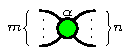
\includegraphics{InclGrphx--generater--green_spider}
			}
			\subcaptionbox{Red spider}[2.5 cm]{%
				\centering
				
\includegraphics{InclGrphx--generater--red_spider}
			}
			\subcaptionbox{Hadamard}[2.5 cm]{%
				\centering
				
\includegraphics[]{InclGrphx--generater--hadamard}
			}
			\subcaptionbox{Diamond}[2 cm]{%
				\centering
				
\includegraphics{InclGrphx--generater--diamond}
			}
			%%%%%%%%%%%%%%%%%%%%%%
		\end{minipage}
	}
	\caption{Generators for the category $\mathbf{zx}$}
	\label{fig:ZX_generators}
\end{figure}
The dangling wires 
on the diagrams' left 
are \emph{inputs} and 
those on the right are \emph{outputs}. 
By connecting inputs to outputs, 
we can form larger diagrams.  
Formalizing this perspective, 
we let these diagrams 
generate the morphisms of 
a dagger compact category 
$\mathbf{zx}$ whose 
objects, the non-negative integers, 
count the inputs and outputs
of a diagram.  
Section 
	\ref{sec:ZxCalc} 
contains a presentation of $\mathbf{zx}$ 
along with a brief discussion on 
the origins of the generating morphisms 
(Figure \ref{fig:ZX_generators}) 
and relations (Figure \ref{fig:ZX_equations}). 
We also mention relevant software, 
Quantomatic 
	\cite{AbramCoecke_CatSemanticQuantum,
		KissingerZamd_Quantomatic} 
and Globular 
	\cite{BarKissingerVicary_Globular}.  

Our goal in this paper is
to generate a
symmetric monoidal and compact closed (SMCC) 
bicategory $\underline{\mathbf{zx}}$
that provides a syntax for the zx-calculus. 
Our first steps towards constructing 
$\underline{\mathbf{zx}}$
is in Section 
	\ref{sec:RewritingOpenGraphs} 
where we fit open graphs 
into an SMCC bicategory.
To this end, 
we slightly modify recent
work by Courser and the author
	\cite{Cicala_SpansCospans,
		CicalaCourser_BicatSpansCospan}
in order to produce an SMCC bicategory 
with graphs as 0-cells, 
cospans of graphs as 1-cells, 
and certain equivalence classes 
of spans of cospans of graphs as 2-cells
(see Figure \ref{fig:spans_of_cospans}). 
As discussed above, this has an
SMCC sub-bicategory $\mathbf{Rewrite}$
that provides an ambient space 
in which to generate systems 
modeled on open graphs.  

\begin{figure}
	\fbox{%
		\begin{minipage}{\textwidth}
			\centering
			%%%%%%%%%%%%%%%%%%%%%%%%%%%%%%%
			\subcaptionbox{A span of cospans}[5cm]{%
				\centering				
				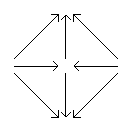
\includegraphics{InclGrphx--SpCsp--span_cospans}
			}
			\subcaptionbox{A span of cospans morphism}[5cm]{%
				\centering
				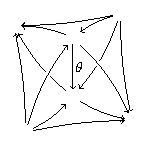
\includegraphics{InclGrphx--SpCsp--map_span_cospans}
			}
			%%%%%%%%%%%%%%%%%%%%%%%%%%%%%%%%
		\end{minipage}
	}
	\caption{A generic $2$-cell in $\mathbf{Sp}(\mathbf{Csp}(C))$}
	\label{fig:spans_of_cospans}
\end{figure}
However, this version of $\cat{Rewrite}$ does not 
contain everything we need.
In Section \ref{sec:OpenGraphsOverSzx}, 
we fill the gap by introducing  
\emph{open graphs over $S_{\text{zx}}$}.  
That is, we pick a graph $S_{\text{zx}}$
\[
	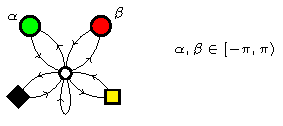
\includegraphics{InclGrphx--slice--graph_S_zx}
\]  
whose nodes coincide with the node types 
found in the zx-calculus diagrams, with
one exception: 
the white node in the center.
This node replaces the
dangling edges in the zx-diagrams. 
A graph morphism $G \to S_{\text{zx}}$ 
then corresponds to a zx-morphism
by transporting the node types to $G$
via the fibres of the map.
In his thesis
	\cite{Kissinger_Pictures}, 
Kissinger also colored
graphs this way.  
We then form an SMCC bicategory with 
graphs over $S_{\text{zx}}$ as 0-cells, 
cospans of graphs over $S_{\text{zx}}$ as 1-cells, 
and spans of cospans as 2-cells.  
These spans of cospans are taken
up to the equivalence relation
obtained by relating 2-cells with the
same domain and codomain.
In analogy to the formation of $\cat{Rewrite}$,
we find a sub-bicategory $\mathbf{zxRewrite}$
that can be thought of as containing all 
open graphs over $S_{\text{zx}}$ and their rewrites.

The bicategory $\mathbf{zxRewrite}$ 
is a space in which we can generate 
SMCC sub-bicategories. 
In Section \ref{sec:zx_categorified}, 
we give a presentation for 
a sub-bicategory $\underline{\mathbf{zx}}$ 
of $\mathbf{zxRewrite}$ whose
1-cells correspond to 
zx-calculus diagrams and
2-cells to the relations between them.  
After constructing $\underline{\mathbf{zx}}$, 
we decategorify it to a 1-category 
$|| \underline{ \mathbf{zx} } ||$ 
by identifying 1-cells whenever 
there is a 2-cell between them.  
Though this seems asymmetrical, 
we actually get an equivalence relation
because of the dual nature of spans.  
In the main result, 
Theorem \ref{thm:equiv_of_zx_cats}, 
we construct a dagger compact functor 
$|| \underline{ \mathbf{zx} } || \to \mathbf{zx}$ 
witnessing an equivalence of categories.  
It is in this sense that we are categorifying
the zx-calculus.

The author would like to thank 
John Baez for many helpful ideas and 
discussions that contributed to this paper. 
A debt of gratitude is also owed
to three anonymous referees for their
insightful comments on
an earlier version of this paper
written for the 2017 Quantum Physics and Logic 
conference in Nijmegen, Netherlands.
